\chapter{Configuración RN4020}\label{rn4020}

\section{BLE (Bluetooth 4.0)}

El módulo de comunicación consiste en el chip RN4020 de MicroChip, el cual opera bajo el estándar BLE (Bluetooth Low Energy). La tecnología BLE consiste en un nuevo estándar de Bluetooth a partir de su versión 4.0, en la cual se optimiza el tamaño y consumo de potencia de los dispositivos, dentro de su implementación cabe mencionar distintos actores y definiciones con los cuales opera:\newline

	-GAP (Generic Access Profile): Dentro de la GAP se definen varios tipos de roles, pero estos están implementados bajo el concepto en que los dispositivos BLE pueden actuar con rol Central o un rol Periférico. Los dispositivos con rol periférico son pequeños, de baja potencia y que pueden conectarse a un dispositivo central mucho más potente. Los dispositivos periféricos pueden ser: monitor de frecuencia cardíaca, una tarjeta de proximidad BLE, etc. Por lo general, los dispositivos con rol Central usualmente son teléfono móvil, tableta o PC los cuales poseen mucha más potencia de procesamiento y memoria.
	
	-GATT (Generic Attribute Profile): Define de qué modo dos dispositivos Bluetooth de bajo consumo transfieren sus datos, haciendo usos de los conceptos de Servicios y Características. Además se hace uso de un protocolo de datos genéricos llamados Attribute Protocol (ATT) en el cual se almacenan los servicio, características y datos relacionados en una simple tabla de consultas en cuya entrada se utiliza un ID de 16 bits. Una vez que ya se encuentra establecida la comunicación entre los dos dispositivos, entra en juego los servicios y atributos definidos por GATT, es decir, que ya tuvo que haber concluido la etapa de Anuncio y asociación de los dispositivos gobernado por las definiciones establecidas por GAP. Cabe mencionar que los servicios y características descritas en la GATT, la conexión entre el dispositivo periférico y el central es exclusiva, es decir, que solo puede haber una comunicación a la vez. De esta manera, para que otro dispositivo pueda conectarse al periférico, primero debe desconectarse de su enlace actual.
	
	-Anunciación de un dispositivo: Hay dos modos diferentes de realizar el envío de datos en un anuncio GAP : Advertising Data y Scan Response. Los datos enviados en cada uno de los anuncios forman el llamado Payload del mensaje. Ambas cargas son idénticas y pueden almacenar hasta 31 bytes de datos, pero sólo los mensajes de
	advertising son obligatorios para la norma, ya que ésta contiene siempre la información útil que constantemente se está transmitiendo desde el dispositivo periférico al dispositivo central. Los datos de los mensajes Scan response actualmente son opcionales y son utilizados para enviar una secuencia de datos secundaria a pedido del dispositivo central. Esto permite a los desarrolladores de equipos ingresar datos adicionales que se entregan en el momento de realizar el anuncio, como indicar el nombre del dispositivo, por ejemplo.

En la figura \ref{advertising} se puede visualizar el proceso de anuncio por parte de un dispositivo periférico a un equipo central y de cómo entran en juego los mensajes del tipo Advertising data y Scan data. 

\begin{figure}[H]
	\centering
	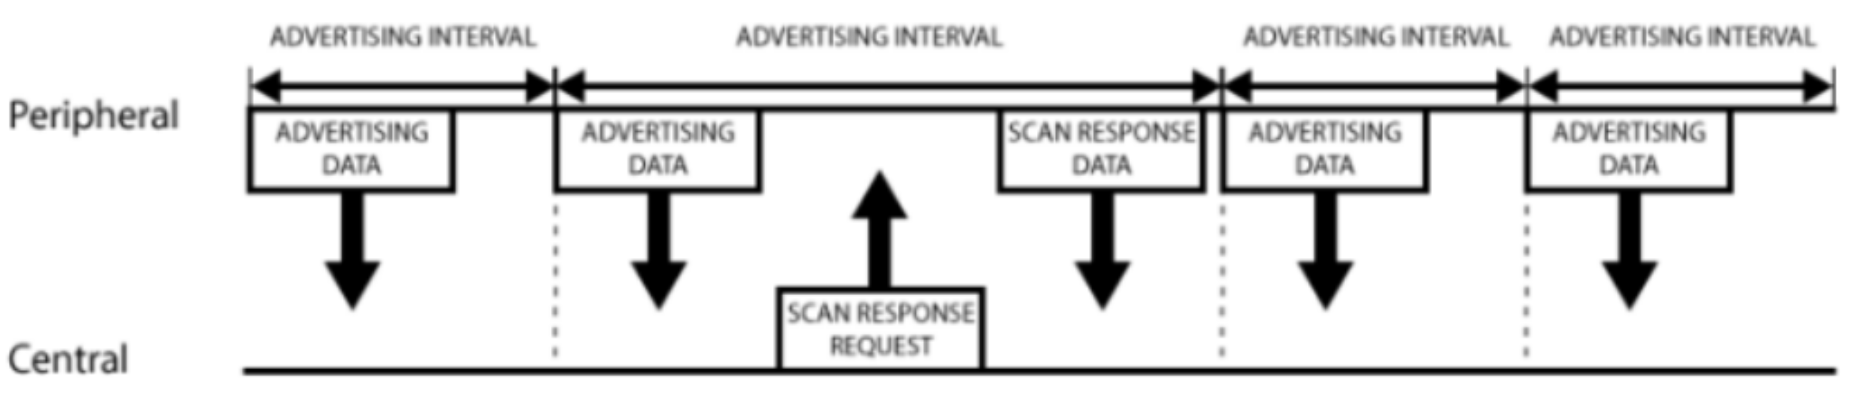
\includegraphics[scale=0.4]{figuras/rn4020/advertising.png}
	\caption{Proceso de anuncio de un dispositivo.}
	\label{advertising}
\end{figure}

Un dispositivo periférico puede definir el intervalo de anuncio, y en cada tiempo en que se alcance este intervalo de anuncio, se enviará un paquete de datos llamado Advertising data. A intervalos largos de anuncios, el dispositivo reduce considerablemente el consumo, pero el equipo es menos sensible a las respuestas si el intervalo de anuncio es de 2 segundos en lugar de 20ms. Si algunos de los dispositivos que se encuentran escuchando estos mensajes de anuncio por parte del periférico está interesado en recibir los datos que agrega el mensaje Scan Payload (y a su vez está disponible en el dispositivo periférico), entonces es posible enviar un mensaje que indica que se requiere el Scan Payload del dispositivo, a lo cual este le responderá con los datos solicitados.

-Transacciones GATT: Un concepto importante para entender GATT es la relación servidor / cliente. El periférico se conoce como el servidor GATT, ya que contiene los datos de búsqueda ATT y las definiciones de servicio y características, y el cliente GATT (el teléfono / tableta), que envía solicitudes a este servidor. 

Al establecer una conexión, el periférico sugerirá un "Intervalo de conexión" al dispositivo central, y el dispositivo central intentará volver a conectar en cada intervalo de conexión para ver si hay nuevos datos disponibles. Es importante tener en cuenta que este "Intervalo de conexión" es sólo una sugerencia, puesto que es posible que el dispositivo central no pueda cumplir con la solicitud porque está ocupado hablando con otro periférico o los recursos del sistema necesarios no están disponibles.

El siguiente diagrama ilustra el proceso de intercambio de datos entre un periférico (el servidor GATT) y un dispositivo central (el cliente GATT), con el dispositivo maestro iniciando cada transacción GATT.\newline

\begin{figure}[H]
	\centering
	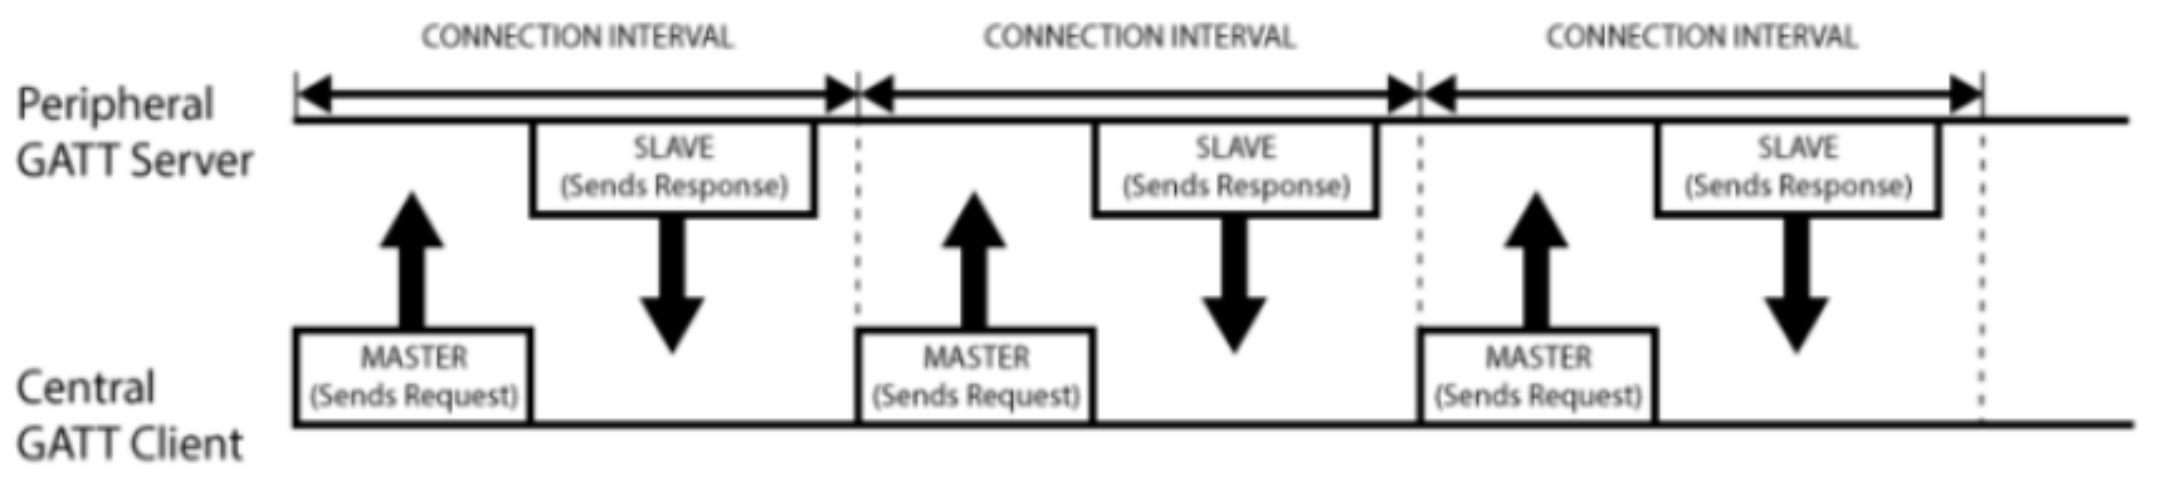
\includegraphics[scale=0.4]{figuras/rn4020/gatt.png}
	\caption{Transacciones GATT.}
	\label{gatt}
\end{figure}



-Perfiles, Servicios, Características y Descriptores: Las transacciones GATT en los dispositivos BLE están basadas en objetos anidados de alto nivel que se denominan Perfiles, Servicios y Características. El orden de estos elementos se muestra a continuación.

\begin{figure}[H]
	\centering
	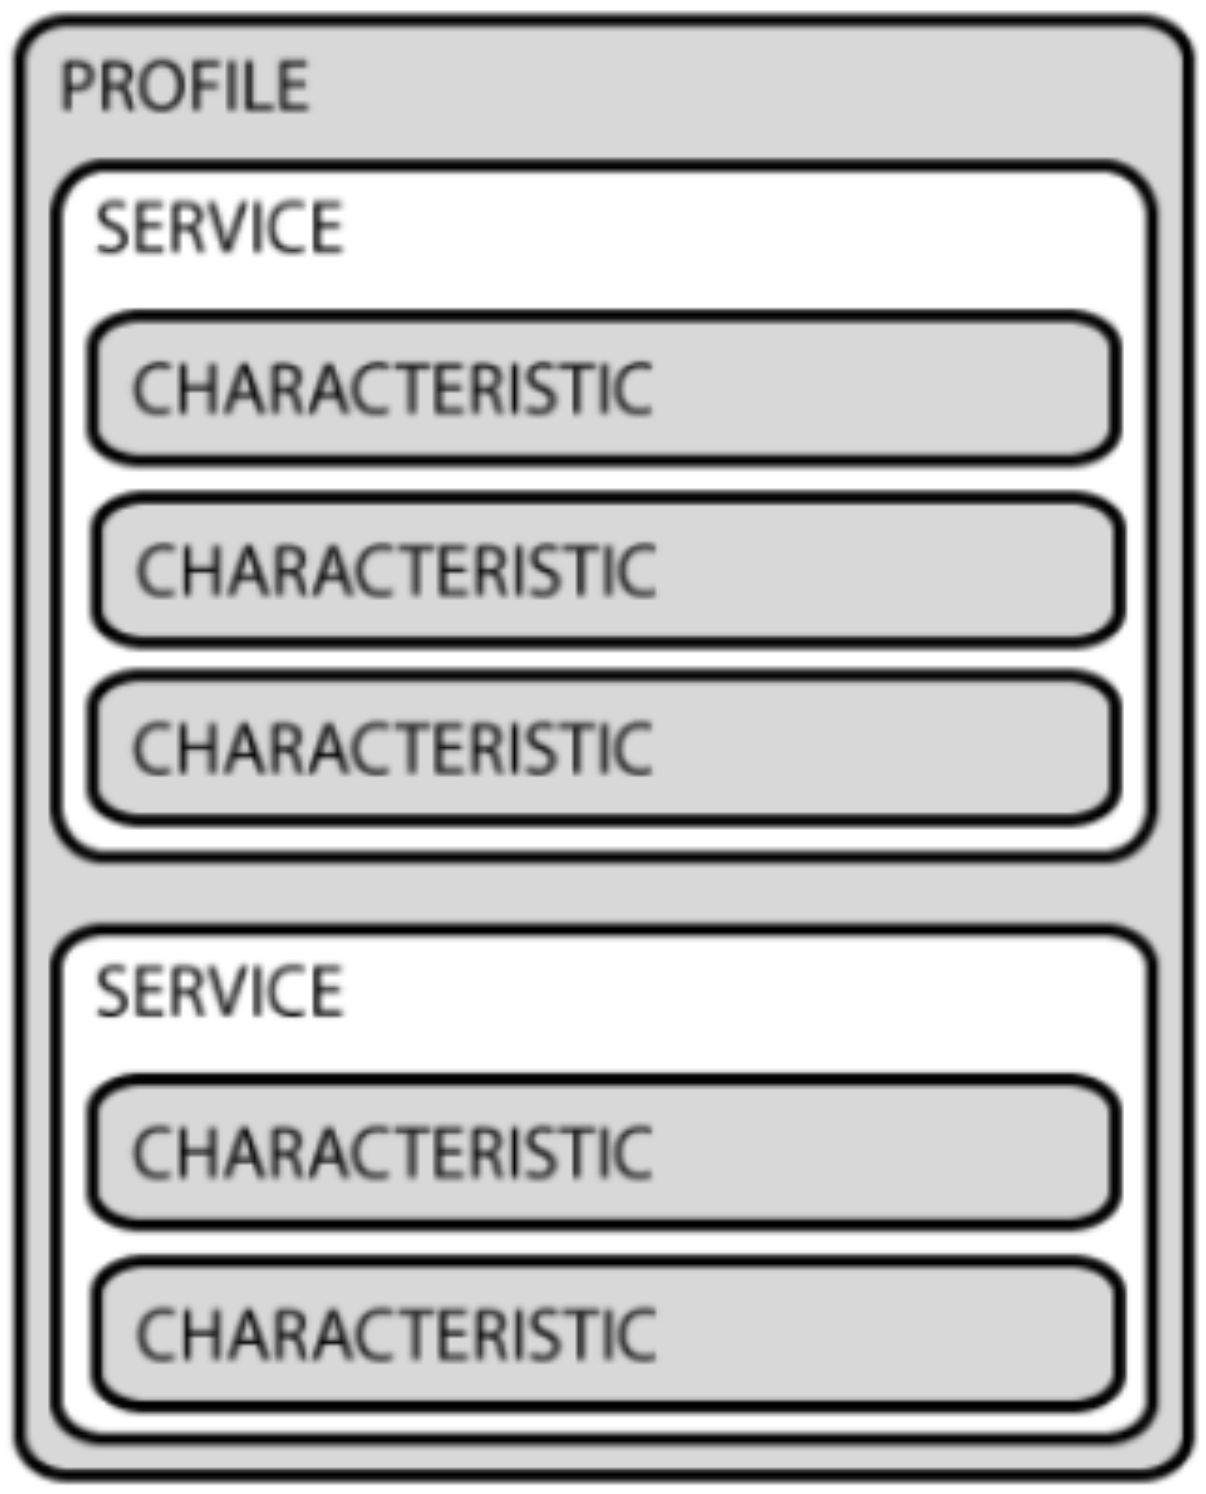
\includegraphics[scale=0.4]{figuras/rn4020/orden_gatt.png}
	\caption{Orden de objetos en transacciones GATT.}
	\label{orden_gatt}
\end{figure}

Un perfil no existe en el propio periférico BLE, sino que es una colección predefinida de servicios que ha sido compilada por el SIG de Bluetooth o por los diseñadores periféricos. El perfil de frecuencia cardiaca, por ejemplo, combina el servicio de frecuencia cardiaca y el servicio de información de dispositivos.\newpage
Los servicios se utilizan para dividir datos en entidades lógicas y contienen porciones específicas de datos llamados Características. Un servicio puede tener una o más características y cada servicio se distingue de otros servicios por medio de un ID numérico único denominado UUID, que puede ser de 16 bits (para servicios BLE adoptados oficialmente) o de 128 bits (para servicios personalizados). Una lista completa de los servicios BLE adoptados oficialmente se puede ver en la página Servicios del Portal de Desarrolladores de Bluetooth.\newline \newline
El concepto de nivel más bajo en las transacciones GATT son las características, que encapsula un único punto de datos (aunque puede contener una matriz de datos relacionados, como valores X / Y / Z de un acelerómetro de 3 ejes, etc.). De forma similar a los Servicios, cada Característica se distingue a través de un UUID predefinido de 16 bits o 128 bits. También se utilizan para enviar datos al periférico BLE, ya que también se puede escribir en la característica. Se puede implementar una interfaz UART simple con un 'Servicio UART' personalizado y dos características, una para el canal TX y otra para el canal RX, donde una característica puede configurarse como de sólo lectura y la otra tiene privilegios de escritura.
Una Característica contiene un único valor y entre 0 y n descriptores que describen el valor de la característica, vale decir, algún rango aceptable o la unidad en caso de ser un valor cuantitativo, hasta una breve descripción de texto. \newpage

-Topología de red a utilizar: Un periférico sólo puede conectarse a un solo dispositivo central (Como un teléfono móvil) a la vez, pero un dispositivo central puede conectarse a varios periféricos. Una vez ya se estableció la conexión entre un dispositivo periférico y un central, la comunicación puede ser bidireccional. Para los fines del proyecto se espera solo una conexión 1 a 1, pero se destaca la comunicación bidireccional posible con este estándar.

\begin{figure}[H]
	\centering
	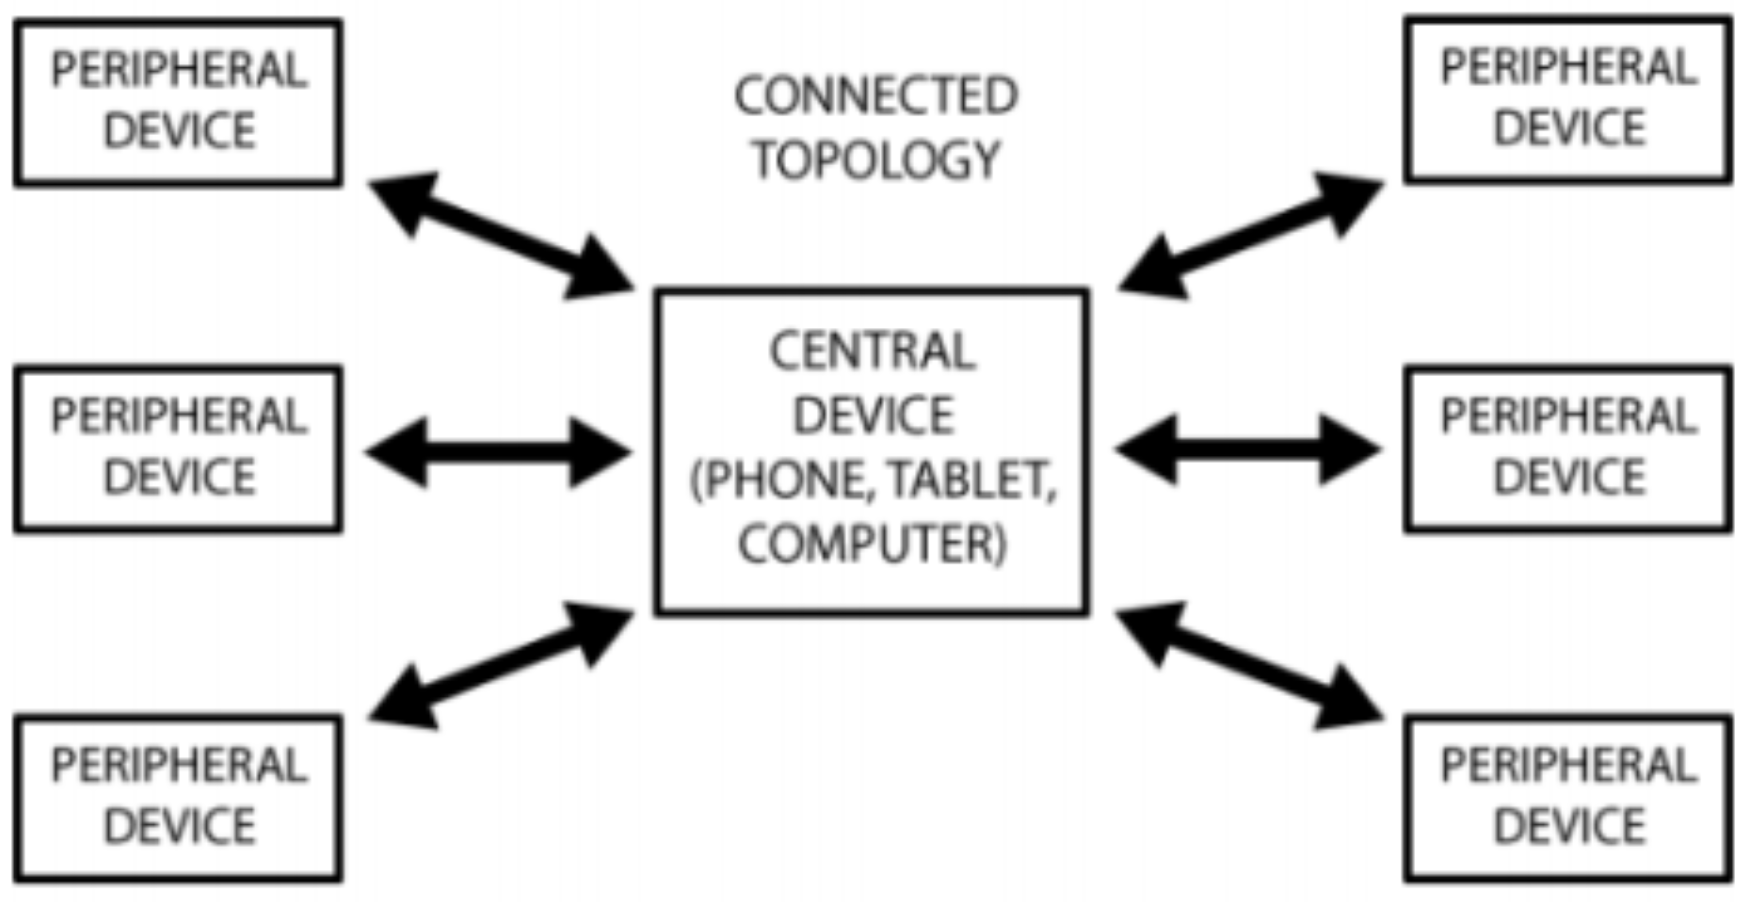
\includegraphics[scale=0.4]{figuras/rn4020/topologia.png}
	\caption{ Topología de red de dispositivos conectados.}
	\label{topologia}
\end{figure}

\newpage

\section{Características disponibles y selección, autoconexión Bluetooth (desde Android)}

Para definir la comunicación Bluetooth con el chip RN4020 (con perfiles GATT) según lo establecido para el proyecto, se hace necesaria la creación de un perfil, servicios y características privadas. Por esto se definen los parámetros a continuación:

Comando: 

	PZ: Limpiar servicios
	
	R,1: Reinicio

	SF,1 y R,1: Restablecer de fábrica

	SR,20402000 y R,1: Características de chip RN4020

	SS,00000001 yR,1: Habilitación de Servicios Privados

	PS,66ecf52ce19f11e48a001681e6b88ec1: Servicio con UUID (random) privada

	PC,UUID,10,01,01 y R,1: Característica asociada a servicio previo

	SUW,UUID,01: Escritura en característica asociada

La mayoría de opciones es utilizada bajo codificación hexadecimal, como lo son tamaños y ciertas características. A partir del o anterior se establecen 2 formas de reconexión: 

	Auto anuncio: El dispositivo BLE al terminar una conexión automáticamente se hace visible.

	Anuncio manual: El dispositivo BLE requiere de una señal para hacerse visible (con la capacidad de recibir otra instrucción para dejar de serlo).

Se decide usar la segunda opción dado que se optimiza el recurso energético y dota de seguridad al dispositivo al no permitir conectarse a cualquiera sin previa interacción directa con el mismo. Además, se utiliza lo aprendido en el capítulo anterior (Servicios en Android para reconexión) para bajo la documentación del chip RN4020 comunicar (bajo notificaciones que no requieren peticiones del cliente Android) el dispositivo BLE con la aplicación. Cabe destacar que la reconexión se puede hacer automática al especificar la conexión GATT, pero esta demora alrededor de 10 segundos.
